\section{lemma3(core)}
\begin{lemma}
\end{lemma}
Suppose we have a Riemann sphere $C$ and two diagrams $(C,\iota,\xi)$,$(C,\iota',\xi')$ and their refinements $\overline{(C,\iota,\xi)}$,$\overline{(C,\iota',\xi')}$ and sheaves $\mathfrak{F}$,$\mathfrak{F}'$ on them such that they differ only on a small disk $D\subset C$. \\

Below figures show only $\mathfrak{F}$, $\mathfrak{F}'$ restricted to $D$.


\begin{figure}[H] % Optional: [h] means here, [t] for top, [b] for bottom, [p] for page of floats
    \centering
    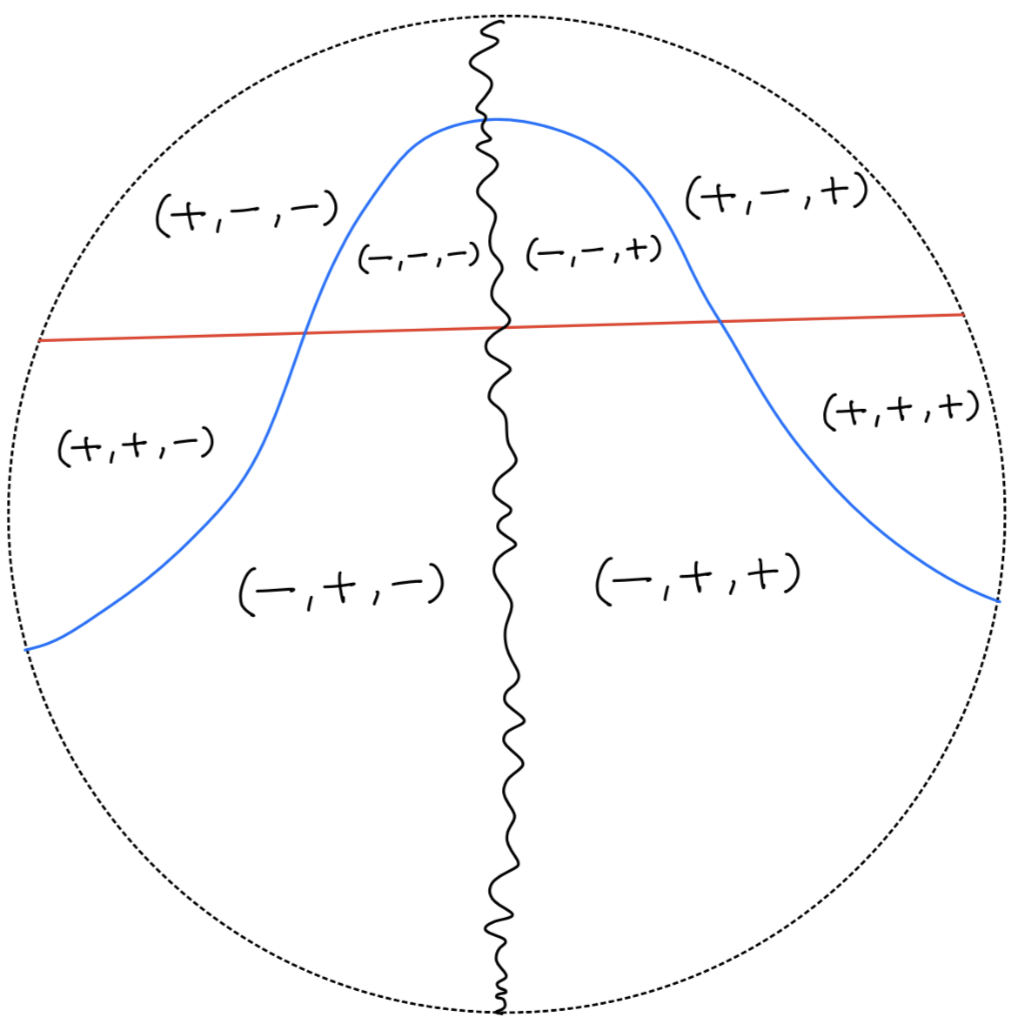
\includegraphics[width=\linewidth]{diagrams/lemma3/1.png} % Adjust the width as needed
    \caption{Your caption here}
    \label{fig:your-label}
\end{figure}

Stalks :\\

- 1 : $\mathbb{C}^{m+1}$\\
- 2 : $\mathbb{C}^{m}$\\
- 3 : $\mathbb{C}^{m}$\\
- 4 : $\mathbb{C}^{m+1}$\\
- 5 : $\mathbb{C}^{m+2}$\\
- 6 : $\mathbb{C}^{m+1}$\\
- 7 : $\mathbb{C}^{m+1}$\\
- 8 : $\mathbb{C}^{m+2}$\\

Generization maps : \\

- 2$\rightarrow$1 : $\iota_l$\\
- 6$\rightarrow$5 : $\iota_l$\\
- 1$\rightarrow$4 : $\iota_l$\\
- 1$\rightarrow$5 : $\iota_f$\\
- 2$\rightarrow$6 : $\iota_f$\\
- 1$\rightarrow$4 : $f$\\
- 2$\rightarrow$3 : $g$\\
- 6$\rightarrow$7 : $h$\\
- 3$\rightarrow$4 : $h'$\\
- 7$\rightarrow$8 : $g'$\\
- 3$\rightarrow$7 : $h''$\\
- 4$\rightarrow$8 : $f''$\\

\begin{figure}[H] % Optional: [h] means here, [t] for top, [b] for bottom, [p] for page of floats
    \centering
    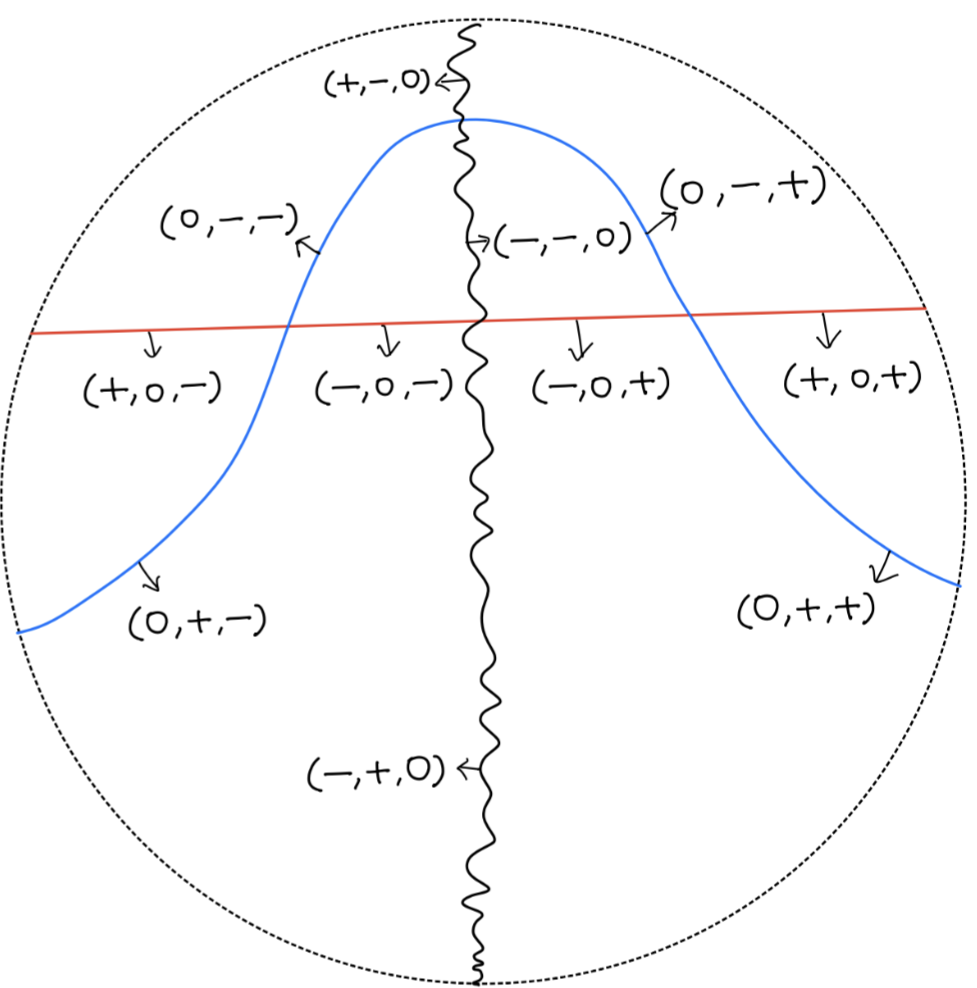
\includegraphics[width=\linewidth]{diagrams/lemma3/2.png} % Adjust the width as needed
    \caption{Your caption here}
    \label{fig:your-label}
\end{figure}

Stalks :\\

- 1 : $\mathbb{C}^{m+1}$\\
- 2 : $\mathbb{C}^{m+2}$\\
- 3 : $\mathbb{C}^{m+1}$\\
- 4 : $\mathbb{C}^{m+1}$\\
- 5 : $\mathbb{C}^{m+2}$\\
- 6 : $\mathbb{C}^{m+1}$\\

Generization maps : \\
- 1$\rightarrow$3 : $\iota_f$\\
- 2$\rightarrow$4 : $\iota_f$\\
- 5$\rightarrow$3 : $\iota_l$\\
- 6$\rightarrow$4 : $\iota_l$\\
- 1$\rightarrow$2 : $f$\\
- 5$\rightarrow$6 : $g$\\
- 2$\rightarrow$4 : $f'$\\
- 6$\rightarrow$4 : $g'$\\
- 3$\rightarrow$4 : $T$\\

where \\
- $T_{(1,1),(m+2,m+1)} = f'\circ f$\\
- $T_{(1,2),(m+2,m+2)}=g'\circ g$\\

We define an isotopy between $\mathfrak{F}$ and $\mathfrak{F}'$ called $isotopy_3$ as follows :\\

$(\Rn{1})$ The trajectory of red strand in $D\times [0,1]$ is $\{(x,y,t)\in D\times [0,1]~|~ y =\frac{1}{2}\}$\\

$(\Rn{2})$ The trajectory of blue strand in $D\times [0,1]$ is $\{(x,y,t)\in D\times [0,1]~|~ y =\frac{5}{3}(t-1)x^2 - \frac{5}{4}+\frac{3}{4}\}$. When $t=t_0$, the above set is a parabola passing through $(-\frac{\sqrt{3}}{2}, -\frac{1}{2})$, $(\frac{\sqrt{3}}{2}, -\frac{1}{2})$, $(0, -\frac{5}{4}t_0 + \frac{3}{4})$\\

$(\Rn{3})$ The trajectory of squiggly line in $D\times [0,1]$ is $\{(x,y,t)\in D\times [0,1]~|~ x =0\}$\\

Now we will describe the sheaf isotopy from $\mathfrak{F}$ to $\mathfrak{F}'$ by assigning stalks to the 8 regions separated by $(\Rn{1},\Rn{2},\Rn{3})$ and generization maps between them.\\

First let's list the 8 regions :\\

1. $\{(x,y,t)\in D\times [0,1]~|~ y \geq \frac{5}{3}(t-1)x^2 - \frac{5}{4} + \frac{3}{4}, y \geq \frac{1}{2}, x\leq 0\}$\\

2. $\{(x,y,t)\in D\times [0,1]~|~ y \geq \frac{5}{3}(t-1)x^2 - \frac{5}{4} + \frac{3}{4}, y \geq \frac{1}{2}, x\geq 0\}$\\

3. $\{(x,y,t)\in D\times [0,1]~|~ y \leq \frac{5}{3}(t-1)x^2 - \frac{5}{4} + \frac{3}{4}, y \geq \frac{1}{2}, x\leq 0\}$\\

4. $\{(x,y,t)\in D\times [0,1]~|~ y \leq \frac{5}{3}(t-1)x^2 - \frac{5}{4} + \frac{3}{4}, y \geq \frac{1}{2}, x\geq 0\}$\\

5. $\{(x,y,t)\in D\times [0,1]~|~ y \geq \frac{5}{3}(t-1)x^2 - \frac{5}{4} + \frac{3}{4}, y \leq \frac{1}{2}, x\leq 0\}$\\

6. $\{(x,y,t)\in D\times [0,1]~|~ y \geq \frac{5}{3}(t-1)x^2 - \frac{5}{4} + \frac{3}{4}, y \leq \frac{1}{2}, x\geq 0\}$

7. $\{(x,y,t)\in D\times [0,1]~|~ y \leq \frac{5}{3}(t-1)x^2 - \frac{5}{4} + \frac{3}{4}, y \leq \frac{1}{2}, x\leq 0\}$\\

8. $\{(x,y,t)\in D\times [0,1]~|~ y \leq \frac{5}{3}(t-1)x^2 - \frac{5}{4} + \frac{3}{4}, y \leq \frac{1}{2}, x\geq 0\}$

Now let's define :\\

Stalks :\\

- 1 : $\mathbb{C}^{m+1}$\\
- 2 : $\mathbb{C}^{m+1}$\\
- 3 : $\mathbb{C}^{m}$\\
- 4 : $\mathbb{C}^{m}$\\
- 5 : $\mathbb{C}^{m+2}$\\
- 6 : $\mathbb{C}^{m+2}$\\
- 7 : $\mathbb{C}^{m+1}$\\
- 8 : $\mathbb{C}^{m+1}$\\

Generization maps : \\

- 3$\rightarrow$1 : $\iota_l$\\
- 7$\rightarrow$5 : $\iota_l$\\
- 1$\rightarrow$5 : $\iota_f$\\
- 3$\rightarrow$7 : $\iota_f$\\
- 1$\rightarrow$2 : $f$\\
- 3$\rightarrow$4 : $h$\\
- 7$\rightarrow$8 : $g$\\
- 4$\rightarrow$2 : $h'$\\
- 8$\rightarrow$6 : $g'$\\
- 4$\rightarrow$8 : $h''$\\
- 2$\rightarrow$6 : $f'$\\
- 5$\rightarrow$6 : $T$\\

Below we will prove that this is a well-defined isotopy between $\mathfrak{F}$ and $\mathfrak{F}'$\\

(proof of well-definedness)